\section{Découpage du projet}

\subsection{IA - Intelligence artificielle}
\setlength{\parindent}{5ex}
Dans l'intérêt de l'intrigue et de l'histoire du jeu, une intelligence artificielle sera utilisée pour contrôler une ou des entités qui tenteront de nuire à notre joueur en réaction à nos choix. Il sera susceptible d'interagir avec l'environnement et le joueur de façon logique afin de fournir un gameplay attrayant.

\subsection{Multijoueur}
\setlength{\parindent}{5ex}
Le mode multijoueur doit permettre à plusieurs joueurs de se rejoindre dans
le même monde qu’en mode solo. Un joueur crée le serveur depuis son jeu et
peut être rejoint par des clients soit sur le même réseau local, auquel cas la
recherche du serveur se fait automatiquement, soit à travers Internet, et dans ce
cas, une adresse IP devra être spécifiée. Il sera possible de rejoindre ou de créer un serveur directement depuis le menu principal du jeu. Cela nécessite donc de créer et de gérer des connexions réseau. Le multijoueur du jeu sera principalement intégré à l'aide de \emph{Unity Lobby} et \emph{Unity Relay}, deux services en \emph{bêta} développés par Unity et intégrés directement dans l'application qui assurent un service multijoueur stable et gratuit.

En s'inspirant de jeux d'horreur tels que \emph{Phasmophobia} ou \emph{Labyrinthine}, Nyctalopia cherche à être un jeu qui intègre un mode multijoueur immersif dans lequel le joueur interagit directement avec les autres joueurs à travers un chat vocal de proximité. Pour se communiquer, le joueur devra se rapprocher des autres joueurs pour être bien entendu. Cette mécanique entraîne des situations dans lesquelles les joueurs se retrouveront seuls, une ressource très utile dans un jeu d'horreur. Le jeu restera bien sûr jouable même sans chat vocal. Le service \emph{Vivox} sera utilisé pour ce faire.

\subsection{Contrôles joueur}
\setlength{\parindent}{5ex}
Le joueur doit pouvoir contrôler le personnage dans la zone de jeu.
Il doit pouvoir se déplacer dans huit directions grâce a une combinaison de quatre touches.
Le joueur doit aussi pouvoir s'accroupir.
Certaines touches dans la partie supérieur du clavier, correspondant aux chiffres, seront assignées à des objets clé du jeu.
Une touche devra permettre au joueur d'ouvrir une carte la zone de jeu.
Ainsi qu'une autre sera assignée à l'action "utiliser" permettant d'interagir 
Le joueur doit pouvoir choisir entre une distribution des touches pour clavier "AZERTY" ou "QWERTY".

\vfill
\noindent\makebox[\linewidth]{\rule{.8\paperwidth}{.6pt}}\\[0.2cm]
EPITA Toulouse - Projet S2 - 2021/2022 \hfill Nyctalopia - gameHUB
\noindent\makebox[\linewidth]{\rule{.8\paperwidth}{.6pt}}

\subsection{Graphismes}
\setlength{\parindent}{5ex}


La plupart des modèles 3D de notre projet proviendront du site officiel \emph{Unity Asset Store}, de \emph{Quixel MegaScans} ou bien seront créés par nos soins grâce à l'outil libre de droit \emph{Blender 3D}.

\subsection{UI/UX - Interface}
\setlength{\parindent}{5ex}
L'interface du jeu est la première chose que les joueurs verront lorsqu'ils ouvriront le jeu. Celui-ci se composera :
\begin{itemize}
    \item - D'un \emph{Boot Screen} :
    \begin{itemize}
        \item - avec le logo Made with Unity (qui pourra être supprimé selon le choix du groupe),
        \item - un avertissement pour les épileptiques,
        \item - le logo du studio.
    \end{itemize}
    \item - D'un \emph{Main Menu} : 
    \begin{itemize}
        \item - avec la possibilité de créer une nouvelle partie,
        \item - de rejoindre un jeu existant,
        \item - de pouvoir accéder au menu options.
    \end{itemize}
    \item - D'un menu \emph{Options} (pour gérer les graphismes, ...).
    \item - Et d'un menu \emph{Pause}.
\end{itemize}

\subsection{Sauvegardes}
\setlength{\parindent}{5ex}
Le joueur devra pouvoir sauvegarder à des points spécifique du jeu à l'aide d'un objet. Ce style de sauvegarde est inspiré des points de sauvegarde des différents jeux vidéos illustrés ci-dessous (\emph{fig. 3} et \emph{fig. 4}).
Ceux-ci seront disposés tout au long du jeu à des points prédéfinis. Trois emplacements de sauvegarde seront disponibles.

\begin{figure}[H]
\centering
\begin{minipage}{.5\textwidth}
  \centering
  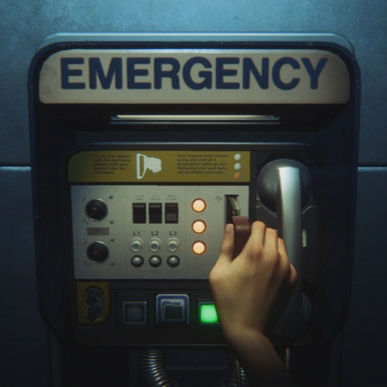
\includegraphics[width=.6\linewidth]{img/savealien.jpg}
  \captionof{figure}{\emph{Alien Isolation}}
  \label{fig:alienisolation}
\end{minipage}%
\begin{minipage}{.5\textwidth}
  \centering
  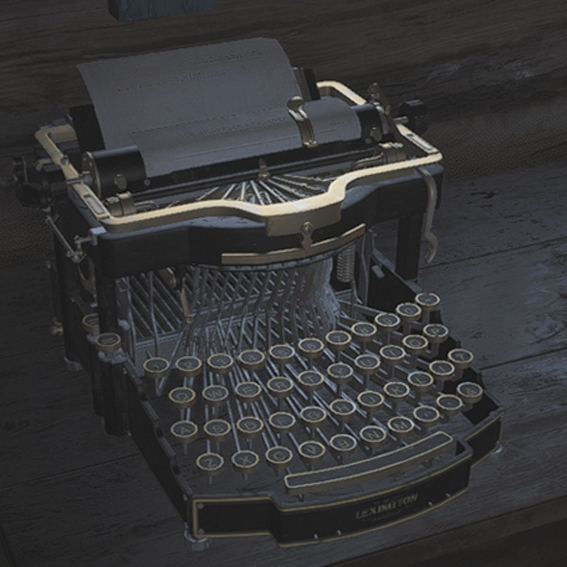
\includegraphics[width=.6\linewidth]{img/savere8.jpg}
  \captionof{figure}{\emph{Resident Evil Village}}
  \label{fig:residentevil8}
\end{minipage}
\end{figure}

\vfill
\noindent\makebox[\linewidth]{\rule{.8\paperwidth}{.6pt}}\\[0.2cm]
EPITA Toulouse - Projet S2 - 2021/2022 \hfill Nyctalopia - gameHUB
\noindent\makebox[\linewidth]{\rule{.8\paperwidth}{.6pt}}

\subsection{Site Web}
\setlength{\parindent}{5ex}
Pour ce projet, le site web sera notre support de promotion. On pourra y télécharger le jeu, les différents manuels d'instruction et d'installation et voir des captures d'écran du jeu. L'équipe de développement sera présentée sur une page, ainsi que tous les logiciels, sons et bibliothèques utilisées. Enfin, le site sera dynamique et utilisera des effets Parallax pour une expérience utilisateur réussie.

Le site web sera hébergé sur CloudFlare Pages, un service gratuit de l'entreprise de gestion DNS CloudFlare, permettant de déployer rapidement à partir d'un repo Git, un site web statique rapide grâce aux serveurs CDN disposés partout dans le monde et sécurisé par un certificat SSL et une protection anti-DDOS.
Le nom de domaine choisi est \emph{nyctalopia.games}. Il est simple et facile à retenir pour l'utilisateur. 

\noindent 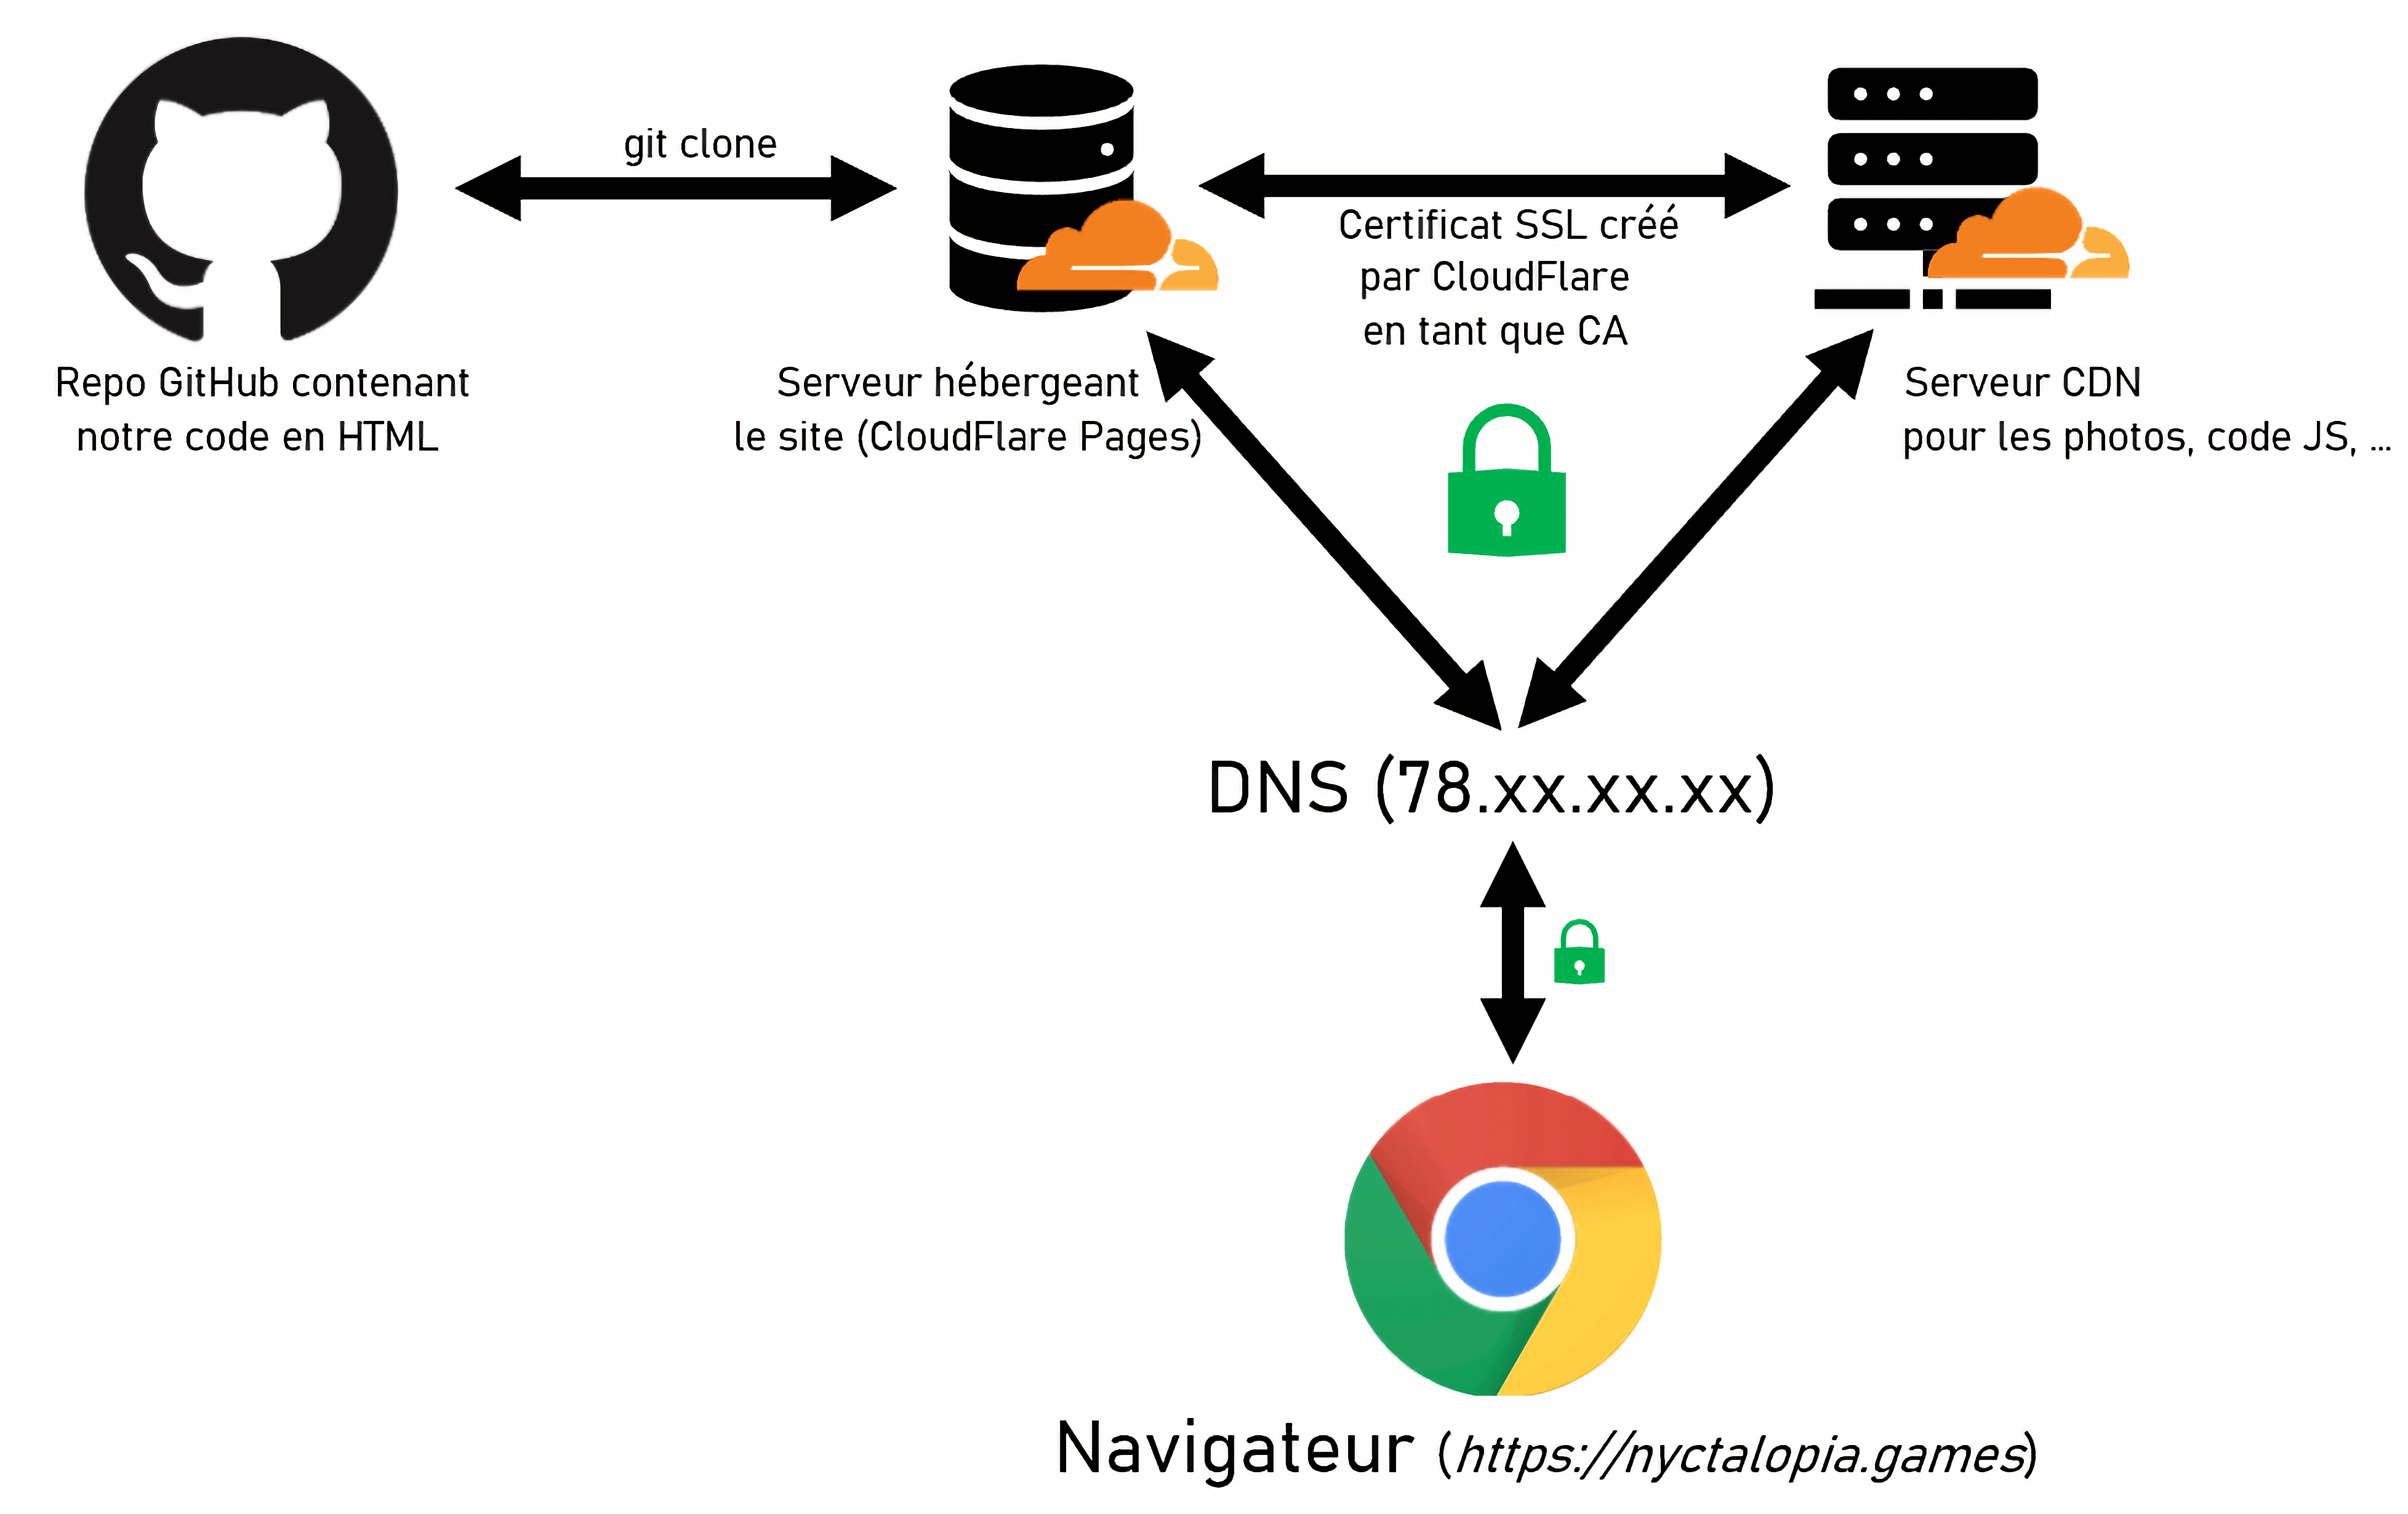
\includegraphics[width=1\linewidth]{img/web.png}
\begin{center}
    FIGURE 6 
    \emph{Schéma simplifié du fonctionnement de notre Site Web}
    \label{fig:web}
\end{center}

\vfill
\noindent\makebox[\linewidth]{\rule{.8\paperwidth}{.6pt}}\\[0.2cm]
EPITA Toulouse - Projet S2 - 2021/2022 \hfill Nyctalopia - gameHUB
\noindent\makebox[\linewidth]{\rule{.8\paperwidth}{.6pt}}

\newpage